\documentclass[12pt]{article}
%%%%%PACKAGES%%%%%
\usepackage[utf8]{inputenc}
\usepackage[T1]{fontenc}
\usepackage{booktabs}
\usepackage{lmodern}
\usepackage{gensymb}
\usepackage{graphicx}
\usepackage{fancyhdr}
\usepackage{geometry}
\usepackage{listings}
\usepackage{tikz}
\usepackage{color, colortbl}
\usepackage{float}
\usepackage{listings}
\usepackage{hyperref}
\usepackage[margin=10pt,font=small,labelfont=bf,labelsep=space]{caption}

\setlength\unitlength{1mm}
\hypersetup{
	colorlinks,
	linkcolor={blue!50!black},
	citecolor={blue!80!black},
	urlcolor={blue!80!black}
}

\definecolor{Gray}{gray}{0.9}
%%%%%%%%%%%%%%%%%%
%%%%%OPTIONS%%%%%%
%%HEADER%%
\pagestyle{fancy}
\lhead{BIO720 Final Project}
\chead{}
\rhead{Yasser Salama}


%%%%%COMMANDS%%%%%
\newcommand{\esal}{\textit{E. salsugenium}}
%%%%%TITLE%%%%%%%%
%Alternate Title%Methodology and Application of Metagenomics for the Characterization of Bacterial Populations in Aquatic Environments
\title{\textsc{Transcriptional Response to Drought Stress in \textit{Eutrema salsugenium}}}
\author{
	{\textsc{\Large Yasser Salama}}\\
	\\
	{McMaster University}\\
	{Hamilton, Ontario, Canada, L8S 4E8}\\
	%{\includegraphics[scale=0.03]{"D:/Dropbox/School/Graduate School/Masters/Thesis/Images/logo_crop"}}
	}
\date{
	{\today}\\
	{\vfill BIO 720 | Bioinformatics}\\
	{Submitted to:}\\
	{Drs. \textsc{Dworkin, Evans, and Golding}}
	}
\begin{document}
	\maketitle
	\thispagestyle{empty}
	\clearpage
	\begin{abstract}
		\pagenumbering{Roman} 
		TEST TEST TEST
	\end{abstract}
	\clearpage
	\tableofcontents
	\listoffigures
	\clearpage
	\section*{Preface}
	The GitHub repository for this report is located \href{https://github.com/salamayg/BIO720}{here.} The repository is set up to contain only the shell, perl, and R scripts used for generating all of the results, as well as the text files containing the count data. The repository does not contain the read files or any subsequent files associated with the reads. The repository is not a clone of the directory on the cluster, however, all the files on the cluster can be accessed (read permission) at /home/yasser/bio720/final\_project. 
	
	When explaining any method or result generated through a script, I will refer to the script in brackets by its names in the scripts folder of the GitHub repository. All the scripts are commented and contain more information about the individual commands than the report will give. 
	\clearpage
	\section{Introduction}
	\pagenumbering{arabic} 
	The prevention of crop loss in the horticulture and agriculture sectors has been a long-standing concern because of the significant economic and societal impacts these losses have. The agriculture industry makes up almost 7\% of Canada's gross domestic product, and with a growing world population, food and water scarcity, and rising global temperatures, these effects will become magnified~\cite{govcan:2015:Online,asseng2015rising,schewe2014multimodel}. 
	
	Abiotic stressors such as drought, salinity, and extreme temperature variations are major drivers of crop loss and can result in 50\% to 80\% loss of crop yield, depending on the crop and growth stage~\cite{boyer1982plant}. Drought is a major facet of abiotic stressors which accounts for approximately 40\% of the indemnities paid for crop loss, larger than any other stressor. As well, in certain crops such as maize and rice, drought alone can account for up to 80\% of the yield loss~\cite{farooq2009plant}. These are extravagant losses with far-reaching impacts. It is therefore imperative to examine the mechanisms by which drought stress can impact plants and their health, and how resistance mechanisms are adapted to such conditions.
	
	The plant response to drought stress is well documented, albeit not fully characterized. In general, the reduction in water availability limits turgidity, inhibiting cell elongation and negatively impacting morphology~\cite{farooq2009plant}. As well, limited nutrient availability, photosynthetic deficits, and consequently diminished mitosis directly impact the health of the plant. 
	The mechanisms by which plants can resist against drought can vary greatly, but typically, there is an attempt to reduce the water requirement through reduced leaf number and surface area, and maximize water uptake through root proliferation. Physiological responses also result in protection against oxidative stress which arise from the generation of reactive oxygen species. These mechanisms involve elevated expression of enzymatic constituents for oxidative stress protection~\cite{farooq2009plant}. Overall, the stress response and resistance mechanisms are extremely complex, and encompass a variety of biological mechanisms. 
	
	The complexity of the stress response is supplemented by the finding that over-expression of known stress-responsive genes typically has little effect on mitigating the stressors' impact. This is likely attributed to the network and co-regulatory nature of the stress response, and requires a more comprehensive understanding of the underlying molecular and physiological changes which occur in response to stress. A useful tool for understanding the stress response and the mechanisms by which it manifests is to examine the complete transcriptional regulation network and the changes that occur once a stress is applied. For the example of drought stress, restriction of water and subsequent comparative examination of the transcriptional changes which occur may provide great insight into the mechanisms for the stress response, and in the case of a drought-tolerant organism, the drought resistance mechanism. 
	
	\textit{Eutrema salsugineum} is a halophytic plant, capable of thriving in various abiotic stress conditions, and is an ideal organism to study the response and resistance mechanism to drought. \esal{} is closely related to the well studied model plant \textit{Arabidopsis thaliana}, with an estimated divergence time of around 43 million years (Figure \ref{phylo}). An important physiological adaptation in \esal{} is the presence of a low permeability cuticle, which reduces the loss of water through the leaves. This waxy cuticle has been observed to be much more abundant in \esal{} than \textit{A. thaliana}, suggesting that this is an adaptive trait for drought resistance. 
	
		\begin{figure}[H]
			\centering
			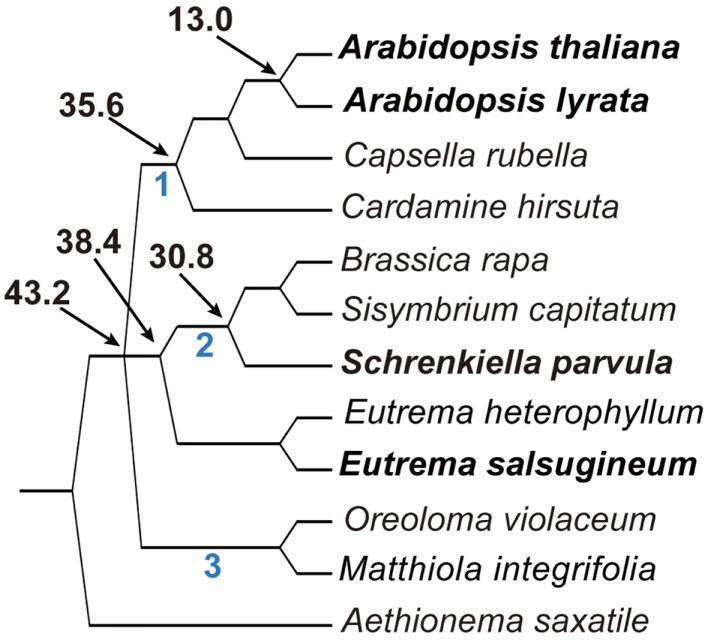
\includegraphics[scale=2]{../figures/esal_phylo.jpg}
			\caption[Brassicaceae Phylogeny]{Brassicaceae phylogeny inferred with two markers, \textit{ndhF} and \textit{PHYA}~\cite{yang2013reference}.}
			\label{phylo}
		\end{figure}
		
	Intriguingly, two different ecotypes of \esal{}, Shandong and Yukon, exist, with different standard environmental conditions. Whereas the Yukon ecotype is sustained in sub-arctic temperatures and a semi-arid climate, the Shandong region is more temperate, although both regions feature a high salinity soil. These two ecotypes show distinct responses to drought stress \cite{xu2014leaf}. Previous findings have shown that the Shandon ecotype seems to have a delayed response to drought and differential changes in cuticle permeability traits between the two ecotypes~\cite{macleod2015exposure}. 
	
		\begin{figure}[H]
			\centering
			\includegraphics[scale=0.2]{../figures/esal_morpho.png}
			\caption[Shandong and Yukon ecotype morphology]{Shandon and Yukon accessions of \esal{}.}
			\label{morpho}
		\end{figure}
		
	The underlying reasons for the differential stress response and resistance of these two ecotypes is not well characterized, and provides a great opportunity to possibly elucidate the molecular mechanisms through which drought is tolerated in plants. By examining the transcriptional adjustments \esal{} undergoes in response to stress, we may begin to understand what pathways are important for this process. By examining two different ecotypes, we can also identify common mechanisms and mechanisms unique to each accession, which is quite informative. 
	
	In this work, we examine the transcriptional response of both \esal{} ecotypes to drought through RNA-seq analysis of Shandon and Yukon ecotypes of \esal{} in well-watered and drought treated conditions. We also examine how the recovery of these plants manifests through a re-watering phase. 


	Establish challenges and the impact of these challenges. Explain that having a model that may provide a foundation of understanding for bypassing these challenges is obviously extremely useful and is needed. Introduce E salsugineum as such a model. Describe it and then the ecotypes and then what is known already. Then describe about what is not known (how the ecotypes differ) and how understanding this can help such agricultural challenges. Describe how you did it, and then a brief overview of the findings.
	
	

	\section{Methods}
	\label{methods}
	\subsection{Plant Growth and Drought Simulation}
	\esal{} seeds corresponding to Yukon (Y) and Shandong (S) accessions were grown at 4\degree C for 4 and 7 days, respectively, to synchronize germination. Subsequently, pots were transferred to growth cabinets simulating standard growth conditions with an optimal watering schedule. The plants were grown under these conditions for 4 weeks after which the plants underwent exposure to drought simulation through complete water-restriction. Effects of the water-restriction were measured gravimetrically using the fraction of transpirable soil water (FTSW) metric. When the fraction reached 0\% (i.e. no remaining water in soil), the plants visibly wilted. Re-watering commenced on the day of wilting to 50\% of the soil capacity, followed by full saturation the next day. Tissue from plants undergoing normal growth conditions (WW, well-watered), drought conditions (D, drought), and re-watering conditions (RW, re-watered) was collected and total RNA was then isolated and processed for sequencing. 
	

	%notes
	the genome is shandong. checked reads mapped.
	only looked at leaves not roots which have the most response to drought
	243 mb genome (check this)
	overexpression of gene induced in stress response has little effect, so its complex. critical reviews in plant sciences
	coverage of mapped reads?
	%notes
	\subsection{Sequencing and RNA-seq Pipeline}
	Two replicates of each treatment and ecotype were used in this analysis, resulting in 12 total samples. Sequencing was completed on a HiSeq 2000 in four batches. A subset of the samples were split onto two lanes, while the rest were run solely on one lane (multiple lane samples are denoted by L1 and L2, see Table \ref{table:samples}). 
	
	\begin{table}[H]
		\centering
		\begin{tabular}{lllrrr}
			\toprule
			Sample & Ecotype & Treatment & Replicate & Lane & Batch\\
			\midrule
			\rowcolor{Gray}
			SD-1 & Shandong & Drought & 1 & 2 & 2\\
			SD-2 & Shandong & Drought & 2 & 2 & 2\\
			\rowcolor{Gray}
			SRW-1.L1 & Shandong & Re-watered & 1 & 1 & 4\\
			\rowcolor{Gray}
			SRW-1.L2 & Shandong & Re-watered & 1 & 2 & 4\\
			SRW-2.L1 & Shandong & Re-watered & 2 & 1 & 4\\
			SRW-2.L2 & Shandong & Re-watered & 2 & 2 & 4\\
			\rowcolor{Gray}
			SWW-1 & Shandong & Well-watered & 1 & 2 & 2\\
			SWW-3.L1 & Shandong & Well-watered & 3 & 1 & 3\\
			SWW-3.L2 & Shandong & Well-watered & 3 & 2 & 3\\
			\rowcolor{Gray}
			YD-1 & Yukon & Drought & 1 & 3 & 1\\
			YD-2.L1 & Yukon & Drought & 2 & 1 & 3\\
			YD-2.L2 & Yukon & Drought & 2 & 2 & 3\\
			\rowcolor{Gray}
			YRW-1 & Yukon & Re-watered & 1 & 3 & 1\\
			YRW-2.L1 & Yukon & Re-watered & 2 & 1 & 3\\
			YRW-2.L2 & Yukon & Re-watered & 2 & 2 & 3\\
			\rowcolor{Gray}
			YWW-1 & Yukon & Well-watered & 1 & 5 & 1\\		
			YWW-2.L1 & Yukon & Well-watered & 2 & 1 & 3\\
			YWW-2.L2 & Yukon & Well-watered & 2 & 2 & 3\\
			\bottomrule
		\end{tabular}
		\caption[Sample Names and Information]{Sample names and information. Each combination of ecotype and treatment had two replicates, with some samples being run across two lanes. All samples were collectively run in four batches.}
		\label{table:samples}
	\end{table}
	FastQC (v0.11.3) was used to validate read metrics prior to and after trimming~\cite{andrews2010fastqc} (script: Step1\_Concat\_trim.sh). A simple loop through all the generated FastQC output files using
	\begin{lstlisting}
	more */summary.txt | grep FAIL
	\end{lstlisting}
	from the fastqc\_reports/pre\_process/ and fastqc\_reports/post\_process/ folders provides a crude way of seeing which metrics fail.
	
	Quality trimming and adapter removal was accomplished with BBDuk from the BBMap suite~\cite{bbmap} (script: Step1\_Concat\_trim.sh). The reference genome and annotation file for \esal{}~\cite{yang2013reference} were downloaded from Phytozyme (v10.3)~\cite{goodstein2012phytozome}. The reference genome is 241 Mb and corresponds to the Shandong ecotype. STAR (v2.3.2) was used to index the reference genome of \esal{} and map the quality filtered reads to the reference~\cite{dobin2013star} (scripts: Step2\_Index\_ref.sh, Step3\_Align.sh) (Figure~\ref{read_stats}). The alignment file was outputted as a bam file already sorted by coordinated through the flag:
	\begin{lstlisting}
	--outSAMtype BAM SortedByCoordinate
	\end{lstlisting}
	
	The bam file generated is in proper format for use with htseq-count and mitigates the need for subsequent sam to bam conversion and sorting. HTSeq-count(v0.6.1) was used to obtain counts for genes in the genome ~\cite{anders2014htseq} using both union and intersection-nonempty modes (scripts: Step4\_Count\_*). 
	
	Read statistics for number of reads prior to and after trimming, as well as number of successfully mapped, were obtained (scripts: trim\_stats.sh, mapped\_stats.sh, read\_statistics.R). 

	\subsection{Differential Gene Expression Analysis}
	\section{Results}
	\subsection{Sample Information and Read Statistics}
	The samples used in this study are summarized in Table~\ref{table:samples}. Since lane effects may introduce a confounding factor and impact results, all the samples which were run on two lanes were left separated. Another potential confounding factor present in the data is the fact that all the samples weren't run together (i.e. run in different batches). Additionally, the only samples run in batch 4 were SRW-1 and SRW-2, which makes it very difficult to rule out whether this batch introduced a systematic variability not due solely to the sample conditions alone. 
	
	FastQC analysis as described in Section~\ref{methods} suggests that even prior to trimming, read quality was a "pass". The only metrics which are considered as "fail" by FastQC are "Sequence duplication levels" and metrics associated with kmer and sequence content. The duplication levels are expected for RNA-seq data as many copies of the same transcript will be present. The kmer and sequence content also seems to be an artifact of the library prepartion method, which introduces nucleotide biases at the beginning of the sequence. More importantly, the  measures of sequence quailty and adapter contamination pass in all of the samples.
	
		\begin{figure}[H]
			\centering
			\scalebox{0.7}{% Created by tikzDevice version 0.9 on 2015-12-14 00:25:55
% !TEX encoding = UTF-8 Unicode
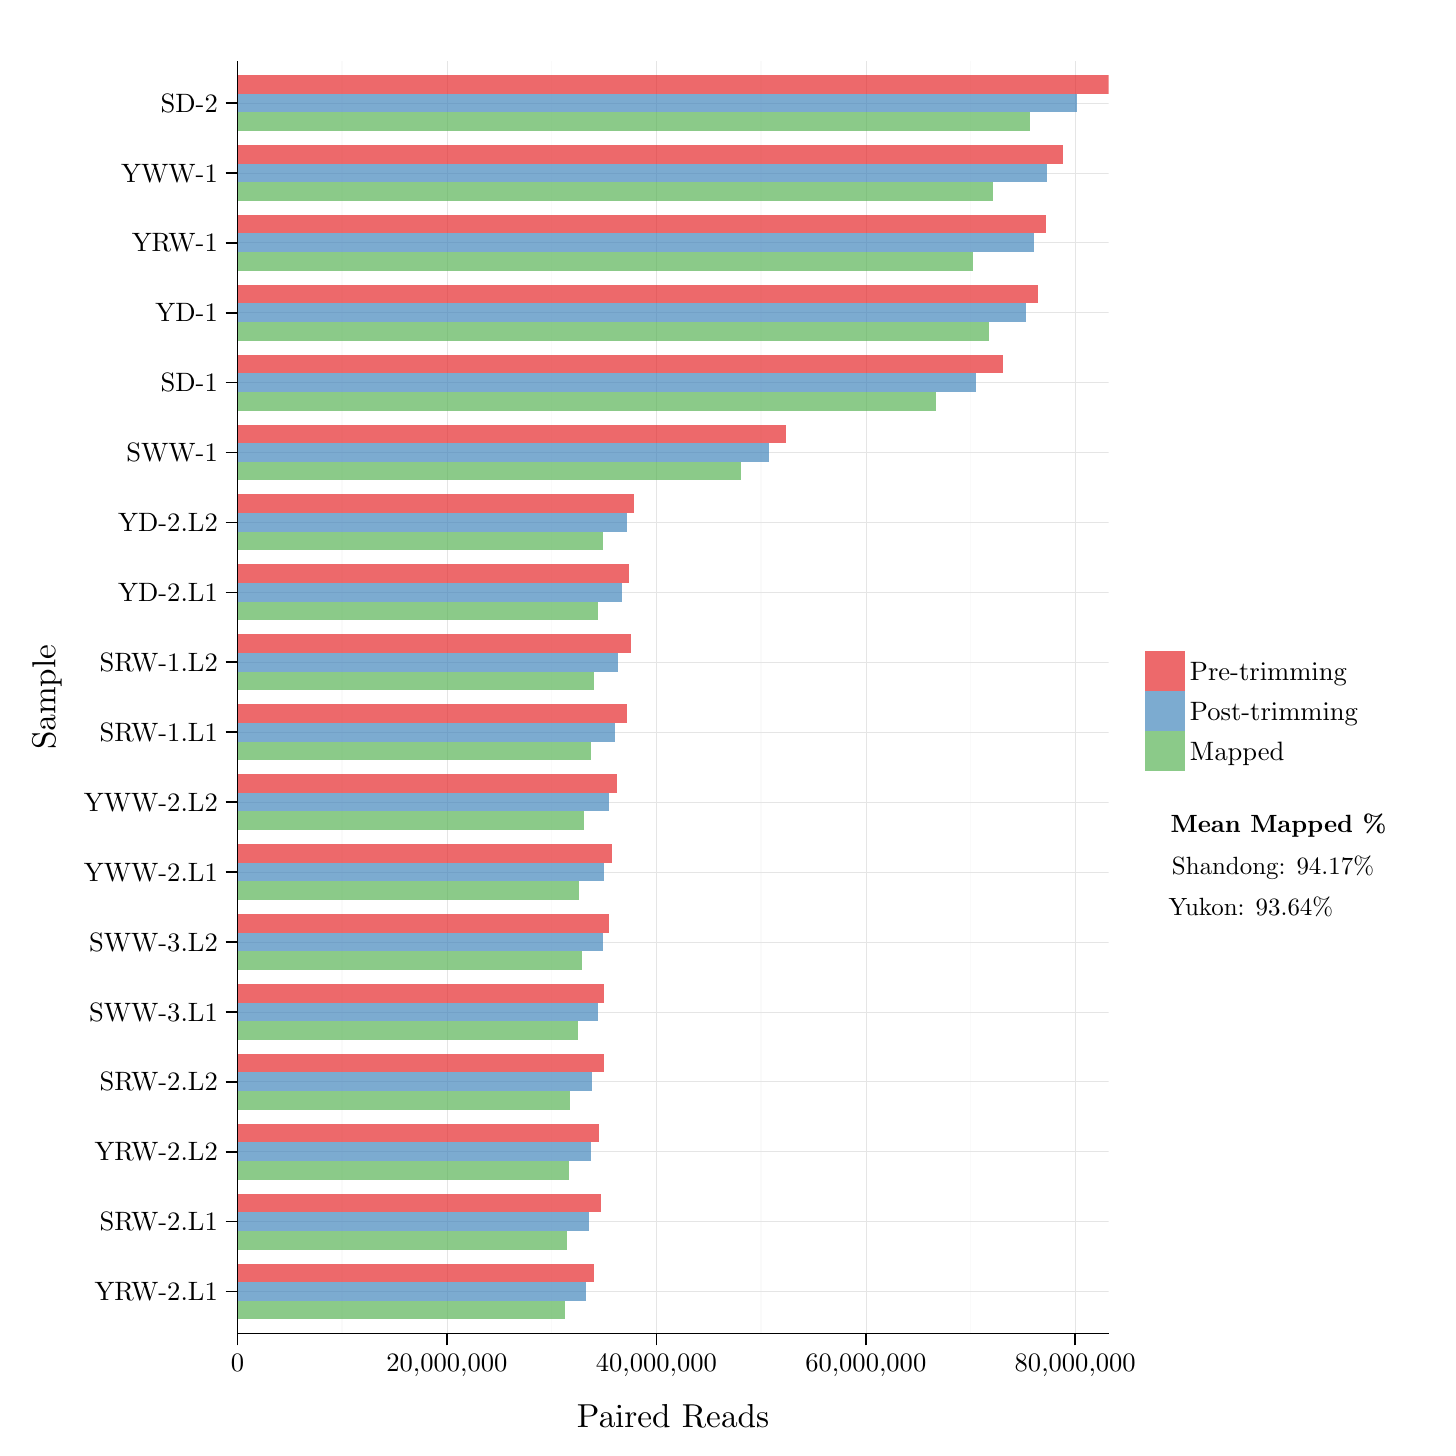
\begin{tikzpicture}[x=1pt,y=1pt]
\definecolor{fillColor}{RGB}{255,255,255}
\path[use as bounding box,fill=fillColor,fill opacity=0.00] (0,0) rectangle (505.89,505.89);
\begin{scope}
\path[clip] (  0.00,  0.00) rectangle (505.89,505.89);
\definecolor{drawColor}{RGB}{255,255,255}
\definecolor{fillColor}{RGB}{255,255,255}

\path[draw=drawColor,line width= 0.6pt,line join=round,line cap=round,fill=fillColor] (  0.00,  0.00) rectangle (505.89,505.89);
\end{scope}
\begin{scope}
\path[clip] ( 75.81, 34.03) rectangle (390.58,493.85);
\definecolor{fillColor}{RGB}{255,255,255}

\path[fill=fillColor] ( 75.81, 34.03) rectangle (390.58,493.85);
\definecolor{drawColor}{gray}{0.98}

\path[draw=drawColor,line width= 0.6pt,line join=round] (113.65, 34.03) --
	(113.65,493.85);

\path[draw=drawColor,line width= 0.6pt,line join=round] (189.33, 34.03) --
	(189.33,493.85);

\path[draw=drawColor,line width= 0.6pt,line join=round] (265.01, 34.03) --
	(265.01,493.85);

\path[draw=drawColor,line width= 0.6pt,line join=round] (340.69, 34.03) --
	(340.69,493.85);
\definecolor{drawColor}{gray}{0.90}

\path[draw=drawColor,line width= 0.2pt,line join=round] ( 75.81, 49.19) --
	(390.58, 49.19);

\path[draw=drawColor,line width= 0.2pt,line join=round] ( 75.81, 74.46) --
	(390.58, 74.46);

\path[draw=drawColor,line width= 0.2pt,line join=round] ( 75.81, 99.72) --
	(390.58, 99.72);

\path[draw=drawColor,line width= 0.2pt,line join=round] ( 75.81,124.99) --
	(390.58,124.99);

\path[draw=drawColor,line width= 0.2pt,line join=round] ( 75.81,150.25) --
	(390.58,150.25);

\path[draw=drawColor,line width= 0.2pt,line join=round] ( 75.81,175.51) --
	(390.58,175.51);

\path[draw=drawColor,line width= 0.2pt,line join=round] ( 75.81,200.78) --
	(390.58,200.78);

\path[draw=drawColor,line width= 0.2pt,line join=round] ( 75.81,226.04) --
	(390.58,226.04);

\path[draw=drawColor,line width= 0.2pt,line join=round] ( 75.81,251.31) --
	(390.58,251.31);

\path[draw=drawColor,line width= 0.2pt,line join=round] ( 75.81,276.57) --
	(390.58,276.57);

\path[draw=drawColor,line width= 0.2pt,line join=round] ( 75.81,301.84) --
	(390.58,301.84);

\path[draw=drawColor,line width= 0.2pt,line join=round] ( 75.81,327.10) --
	(390.58,327.10);

\path[draw=drawColor,line width= 0.2pt,line join=round] ( 75.81,352.36) --
	(390.58,352.36);

\path[draw=drawColor,line width= 0.2pt,line join=round] ( 75.81,377.63) --
	(390.58,377.63);

\path[draw=drawColor,line width= 0.2pt,line join=round] ( 75.81,402.89) --
	(390.58,402.89);

\path[draw=drawColor,line width= 0.2pt,line join=round] ( 75.81,428.16) --
	(390.58,428.16);

\path[draw=drawColor,line width= 0.2pt,line join=round] ( 75.81,453.42) --
	(390.58,453.42);

\path[draw=drawColor,line width= 0.2pt,line join=round] ( 75.81,478.69) --
	(390.58,478.69);

\path[draw=drawColor,line width= 0.2pt,line join=round] ( 75.81, 34.03) --
	( 75.81,493.85);

\path[draw=drawColor,line width= 0.2pt,line join=round] (151.49, 34.03) --
	(151.49,493.85);

\path[draw=drawColor,line width= 0.2pt,line join=round] (227.17, 34.03) --
	(227.17,493.85);

\path[draw=drawColor,line width= 0.2pt,line join=round] (302.85, 34.03) --
	(302.85,493.85);

\path[draw=drawColor,line width= 0.2pt,line join=round] (378.53, 34.03) --
	(378.53,493.85);
\definecolor{fillColor}{RGB}{228,26,28}

\path[fill=fillColor,fill opacity=0.65] ( 75.81, 52.56) rectangle (204.60, 59.30);
\definecolor{fillColor}{RGB}{55,126,184}

\path[fill=fillColor,fill opacity=0.65] ( 75.81, 45.82) rectangle (201.91, 52.56);
\definecolor{fillColor}{RGB}{77,175,74}

\path[fill=fillColor,fill opacity=0.65] ( 75.81, 39.09) rectangle (194.13, 45.82);
\definecolor{fillColor}{RGB}{228,26,28}

\path[fill=fillColor,fill opacity=0.65] ( 75.81, 77.83) rectangle (207.05, 84.56);
\definecolor{fillColor}{RGB}{55,126,184}

\path[fill=fillColor,fill opacity=0.65] ( 75.81, 71.09) rectangle (202.71, 77.83);
\definecolor{fillColor}{RGB}{77,175,74}

\path[fill=fillColor,fill opacity=0.65] ( 75.81, 64.35) rectangle (194.85, 71.09);
\definecolor{fillColor}{RGB}{228,26,28}

\path[fill=fillColor,fill opacity=0.65] ( 75.81,103.09) rectangle (206.30,109.83);
\definecolor{fillColor}{RGB}{55,126,184}

\path[fill=fillColor,fill opacity=0.65] ( 75.81, 96.35) rectangle (203.55,103.09);
\definecolor{fillColor}{RGB}{77,175,74}

\path[fill=fillColor,fill opacity=0.65] ( 75.81, 89.62) rectangle (195.72, 96.35);
\definecolor{fillColor}{RGB}{228,26,28}

\path[fill=fillColor,fill opacity=0.65] ( 75.81,128.35) rectangle (208.32,135.09);
\definecolor{fillColor}{RGB}{55,126,184}

\path[fill=fillColor,fill opacity=0.65] ( 75.81,121.62) rectangle (203.87,128.35);
\definecolor{fillColor}{RGB}{77,175,74}

\path[fill=fillColor,fill opacity=0.65] ( 75.81,114.88) rectangle (196.00,121.62);
\definecolor{fillColor}{RGB}{228,26,28}

\path[fill=fillColor,fill opacity=0.65] ( 75.81,153.62) rectangle (208.39,160.36);
\definecolor{fillColor}{RGB}{55,126,184}

\path[fill=fillColor,fill opacity=0.65] ( 75.81,146.88) rectangle (206.01,153.62);
\definecolor{fillColor}{RGB}{77,175,74}

\path[fill=fillColor,fill opacity=0.65] ( 75.81,140.14) rectangle (198.71,146.88);
\definecolor{fillColor}{RGB}{228,26,28}

\path[fill=fillColor,fill opacity=0.65] ( 75.81,178.88) rectangle (210.22,185.62);
\definecolor{fillColor}{RGB}{55,126,184}

\path[fill=fillColor,fill opacity=0.65] ( 75.81,172.15) rectangle (207.77,178.88);
\definecolor{fillColor}{RGB}{77,175,74}

\path[fill=fillColor,fill opacity=0.65] ( 75.81,165.41) rectangle (200.46,172.15);
\definecolor{fillColor}{RGB}{228,26,28}

\path[fill=fillColor,fill opacity=0.65] ( 75.81,204.15) rectangle (211.03,210.88);
\definecolor{fillColor}{RGB}{55,126,184}

\path[fill=fillColor,fill opacity=0.65] ( 75.81,197.41) rectangle (208.35,204.15);
\definecolor{fillColor}{RGB}{77,175,74}

\path[fill=fillColor,fill opacity=0.65] ( 75.81,190.67) rectangle (199.38,197.41);
\definecolor{fillColor}{RGB}{228,26,28}

\path[fill=fillColor,fill opacity=0.65] ( 75.81,229.41) rectangle (212.92,236.15);
\definecolor{fillColor}{RGB}{55,126,184}

\path[fill=fillColor,fill opacity=0.65] ( 75.81,222.67) rectangle (210.17,229.41);
\definecolor{fillColor}{RGB}{77,175,74}

\path[fill=fillColor,fill opacity=0.65] ( 75.81,215.94) rectangle (201.14,222.67);
\definecolor{fillColor}{RGB}{228,26,28}

\path[fill=fillColor,fill opacity=0.65] ( 75.81,254.68) rectangle (216.64,261.41);
\definecolor{fillColor}{RGB}{55,126,184}

\path[fill=fillColor,fill opacity=0.65] ( 75.81,247.94) rectangle (212.28,254.68);
\definecolor{fillColor}{RGB}{77,175,74}

\path[fill=fillColor,fill opacity=0.65] ( 75.81,241.20) rectangle (203.65,247.94);
\definecolor{fillColor}{RGB}{228,26,28}

\path[fill=fillColor,fill opacity=0.65] ( 75.81,279.94) rectangle (217.84,286.68);
\definecolor{fillColor}{RGB}{55,126,184}

\path[fill=fillColor,fill opacity=0.65] ( 75.81,273.20) rectangle (213.38,279.94);
\definecolor{fillColor}{RGB}{77,175,74}

\path[fill=fillColor,fill opacity=0.65] ( 75.81,266.47) rectangle (204.75,273.20);
\definecolor{fillColor}{RGB}{228,26,28}

\path[fill=fillColor,fill opacity=0.65] ( 75.81,305.20) rectangle (217.17,311.94);
\definecolor{fillColor}{RGB}{55,126,184}

\path[fill=fillColor,fill opacity=0.65] ( 75.81,298.47) rectangle (214.80,305.20);
\definecolor{fillColor}{RGB}{77,175,74}

\path[fill=fillColor,fill opacity=0.65] ( 75.81,291.73) rectangle (206.09,298.47);
\definecolor{fillColor}{RGB}{228,26,28}

\path[fill=fillColor,fill opacity=0.65] ( 75.81,330.47) rectangle (219.12,337.21);
\definecolor{fillColor}{RGB}{55,126,184}

\path[fill=fillColor,fill opacity=0.65] ( 75.81,323.73) rectangle (216.68,330.47);
\definecolor{fillColor}{RGB}{77,175,74}

\path[fill=fillColor,fill opacity=0.65] ( 75.81,316.99) rectangle (207.93,323.73);
\definecolor{fillColor}{RGB}{228,26,28}

\path[fill=fillColor,fill opacity=0.65] ( 75.81,355.73) rectangle (273.87,362.47);
\definecolor{fillColor}{RGB}{55,126,184}

\path[fill=fillColor,fill opacity=0.65] ( 75.81,349.00) rectangle (268.04,355.73);
\definecolor{fillColor}{RGB}{77,175,74}

\path[fill=fillColor,fill opacity=0.65] ( 75.81,342.26) rectangle (257.74,349.00);
\definecolor{fillColor}{RGB}{228,26,28}

\path[fill=fillColor,fill opacity=0.65] ( 75.81,381.00) rectangle (352.57,387.73);
\definecolor{fillColor}{RGB}{55,126,184}

\path[fill=fillColor,fill opacity=0.65] ( 75.81,374.26) rectangle (342.64,381.00);
\definecolor{fillColor}{RGB}{77,175,74}

\path[fill=fillColor,fill opacity=0.65] ( 75.81,367.52) rectangle (328.06,374.26);
\definecolor{fillColor}{RGB}{228,26,28}

\path[fill=fillColor,fill opacity=0.65] ( 75.81,406.26) rectangle (364.93,413.00);
\definecolor{fillColor}{RGB}{55,126,184}

\path[fill=fillColor,fill opacity=0.65] ( 75.81,399.52) rectangle (360.81,406.26);
\definecolor{fillColor}{RGB}{77,175,74}

\path[fill=fillColor,fill opacity=0.65] ( 75.81,392.79) rectangle (347.46,399.52);
\definecolor{fillColor}{RGB}{228,26,28}

\path[fill=fillColor,fill opacity=0.65] ( 75.81,431.53) rectangle (367.82,438.26);
\definecolor{fillColor}{RGB}{55,126,184}

\path[fill=fillColor,fill opacity=0.65] ( 75.81,424.79) rectangle (363.80,431.53);
\definecolor{fillColor}{RGB}{77,175,74}

\path[fill=fillColor,fill opacity=0.65] ( 75.81,418.05) rectangle (341.75,424.79);
\definecolor{fillColor}{RGB}{228,26,28}

\path[fill=fillColor,fill opacity=0.65] ( 75.81,456.79) rectangle (374.26,463.53);
\definecolor{fillColor}{RGB}{55,126,184}

\path[fill=fillColor,fill opacity=0.65] ( 75.81,450.05) rectangle (368.17,456.79);
\definecolor{fillColor}{RGB}{77,175,74}

\path[fill=fillColor,fill opacity=0.65] ( 75.81,443.32) rectangle (348.70,450.05);
\definecolor{fillColor}{RGB}{228,26,28}

\path[fill=fillColor,fill opacity=0.65] ( 75.81,482.05) rectangle (390.58,488.79);
\definecolor{fillColor}{RGB}{55,126,184}

\path[fill=fillColor,fill opacity=0.65] ( 75.81,475.32) rectangle (378.99,482.05);
\definecolor{fillColor}{RGB}{77,175,74}

\path[fill=fillColor,fill opacity=0.65] ( 75.81,468.58) rectangle (362.15,475.32);
\end{scope}
\begin{scope}
\path[clip] (  0.00,  0.00) rectangle (505.89,505.89);
\definecolor{drawColor}{RGB}{0,0,0}

\path[draw=drawColor,line width= 0.6pt,line join=round] ( 75.81, 34.03) --
	( 75.81,493.85);
\end{scope}
\begin{scope}
\path[clip] (  0.00,  0.00) rectangle (505.89,505.89);
\definecolor{drawColor}{RGB}{0,0,0}

\node[text=drawColor,anchor=base east,inner sep=0pt, outer sep=0pt, scale=  0.96] at ( 68.70, 45.89) {YRW-2.L1};

\node[text=drawColor,anchor=base east,inner sep=0pt, outer sep=0pt, scale=  0.96] at ( 68.70, 71.15) {SRW-2.L1};

\node[text=drawColor,anchor=base east,inner sep=0pt, outer sep=0pt, scale=  0.96] at ( 68.70, 96.42) {YRW-2.L2};

\node[text=drawColor,anchor=base east,inner sep=0pt, outer sep=0pt, scale=  0.96] at ( 68.70,121.68) {SRW-2.L2};

\node[text=drawColor,anchor=base east,inner sep=0pt, outer sep=0pt, scale=  0.96] at ( 68.70,146.94) {SWW-3.L1};

\node[text=drawColor,anchor=base east,inner sep=0pt, outer sep=0pt, scale=  0.96] at ( 68.70,172.21) {SWW-3.L2};

\node[text=drawColor,anchor=base east,inner sep=0pt, outer sep=0pt, scale=  0.96] at ( 68.70,197.47) {YWW-2.L1};

\node[text=drawColor,anchor=base east,inner sep=0pt, outer sep=0pt, scale=  0.96] at ( 68.70,222.74) {YWW-2.L2};

\node[text=drawColor,anchor=base east,inner sep=0pt, outer sep=0pt, scale=  0.96] at ( 68.70,248.00) {SRW-1.L1};

\node[text=drawColor,anchor=base east,inner sep=0pt, outer sep=0pt, scale=  0.96] at ( 68.70,273.27) {SRW-1.L2};

\node[text=drawColor,anchor=base east,inner sep=0pt, outer sep=0pt, scale=  0.96] at ( 68.70,298.53) {YD-2.L1};

\node[text=drawColor,anchor=base east,inner sep=0pt, outer sep=0pt, scale=  0.96] at ( 68.70,323.79) {YD-2.L2};

\node[text=drawColor,anchor=base east,inner sep=0pt, outer sep=0pt, scale=  0.96] at ( 68.70,349.06) {SWW-1};

\node[text=drawColor,anchor=base east,inner sep=0pt, outer sep=0pt, scale=  0.96] at ( 68.70,374.32) {SD-1};

\node[text=drawColor,anchor=base east,inner sep=0pt, outer sep=0pt, scale=  0.96] at ( 68.70,399.59) {YD-1};

\node[text=drawColor,anchor=base east,inner sep=0pt, outer sep=0pt, scale=  0.96] at ( 68.70,424.85) {YRW-1};

\node[text=drawColor,anchor=base east,inner sep=0pt, outer sep=0pt, scale=  0.96] at ( 68.70,450.12) {YWW-1};

\node[text=drawColor,anchor=base east,inner sep=0pt, outer sep=0pt, scale=  0.96] at ( 68.70,475.38) {SD-2};
\end{scope}
\begin{scope}
\path[clip] (  0.00,  0.00) rectangle (505.89,505.89);
\definecolor{drawColor}{RGB}{0,0,0}

\path[draw=drawColor,line width= 0.6pt,line join=round] ( 71.54, 49.19) --
	( 75.81, 49.19);

\path[draw=drawColor,line width= 0.6pt,line join=round] ( 71.54, 74.46) --
	( 75.81, 74.46);

\path[draw=drawColor,line width= 0.6pt,line join=round] ( 71.54, 99.72) --
	( 75.81, 99.72);

\path[draw=drawColor,line width= 0.6pt,line join=round] ( 71.54,124.99) --
	( 75.81,124.99);

\path[draw=drawColor,line width= 0.6pt,line join=round] ( 71.54,150.25) --
	( 75.81,150.25);

\path[draw=drawColor,line width= 0.6pt,line join=round] ( 71.54,175.51) --
	( 75.81,175.51);

\path[draw=drawColor,line width= 0.6pt,line join=round] ( 71.54,200.78) --
	( 75.81,200.78);

\path[draw=drawColor,line width= 0.6pt,line join=round] ( 71.54,226.04) --
	( 75.81,226.04);

\path[draw=drawColor,line width= 0.6pt,line join=round] ( 71.54,251.31) --
	( 75.81,251.31);

\path[draw=drawColor,line width= 0.6pt,line join=round] ( 71.54,276.57) --
	( 75.81,276.57);

\path[draw=drawColor,line width= 0.6pt,line join=round] ( 71.54,301.84) --
	( 75.81,301.84);

\path[draw=drawColor,line width= 0.6pt,line join=round] ( 71.54,327.10) --
	( 75.81,327.10);

\path[draw=drawColor,line width= 0.6pt,line join=round] ( 71.54,352.36) --
	( 75.81,352.36);

\path[draw=drawColor,line width= 0.6pt,line join=round] ( 71.54,377.63) --
	( 75.81,377.63);

\path[draw=drawColor,line width= 0.6pt,line join=round] ( 71.54,402.89) --
	( 75.81,402.89);

\path[draw=drawColor,line width= 0.6pt,line join=round] ( 71.54,428.16) --
	( 75.81,428.16);

\path[draw=drawColor,line width= 0.6pt,line join=round] ( 71.54,453.42) --
	( 75.81,453.42);

\path[draw=drawColor,line width= 0.6pt,line join=round] ( 71.54,478.69) --
	( 75.81,478.69);
\end{scope}
\begin{scope}
\path[clip] (  0.00,  0.00) rectangle (505.89,505.89);
\definecolor{drawColor}{RGB}{0,0,0}

\path[draw=drawColor,line width= 0.6pt,line join=round] ( 75.81, 34.03) --
	(390.58, 34.03);
\end{scope}
\begin{scope}
\path[clip] (  0.00,  0.00) rectangle (505.89,505.89);
\definecolor{drawColor}{RGB}{0,0,0}

\path[draw=drawColor,line width= 0.6pt,line join=round] ( 75.81, 29.77) --
	( 75.81, 34.03);

\path[draw=drawColor,line width= 0.6pt,line join=round] (151.49, 29.77) --
	(151.49, 34.03);

\path[draw=drawColor,line width= 0.6pt,line join=round] (227.17, 29.77) --
	(227.17, 34.03);

\path[draw=drawColor,line width= 0.6pt,line join=round] (302.85, 29.77) --
	(302.85, 34.03);

\path[draw=drawColor,line width= 0.6pt,line join=round] (378.53, 29.77) --
	(378.53, 34.03);
\end{scope}
\begin{scope}
\path[clip] (  0.00,  0.00) rectangle (505.89,505.89);
\definecolor{drawColor}{RGB}{0,0,0}

\node[text=drawColor,anchor=base,inner sep=0pt, outer sep=0pt, scale=  0.96] at ( 75.81, 20.31) {0};

\node[text=drawColor,anchor=base,inner sep=0pt, outer sep=0pt, scale=  0.96] at (151.49, 20.31) {20,000,000};

\node[text=drawColor,anchor=base,inner sep=0pt, outer sep=0pt, scale=  0.96] at (227.17, 20.31) {40,000,000};

\node[text=drawColor,anchor=base,inner sep=0pt, outer sep=0pt, scale=  0.96] at (302.85, 20.31) {60,000,000};

\node[text=drawColor,anchor=base,inner sep=0pt, outer sep=0pt, scale=  0.96] at (378.53, 20.31) {80,000,000};
\end{scope}
\begin{scope}
\path[clip] (  0.00,  0.00) rectangle (505.89,505.89);
\definecolor{drawColor}{RGB}{0,0,0}

\node[text=drawColor,anchor=base,inner sep=0pt, outer sep=0pt, scale=  1.20] at (233.20,  0) {Paired Reads};
\end{scope}
\begin{scope}
\path[clip] (  0.00,  0.00) rectangle (505.89,505.89);
\definecolor{drawColor}{RGB}{0,0,0}

\node[text=drawColor,rotate= 90.00,anchor=base,inner sep=0pt, outer sep=0pt, scale=  1.20] at ( 10,263.94) {Sample};
\end{scope}
\begin{scope}
\path[clip] (  0.00,  0.00) rectangle (505.89,505.89);
\definecolor{fillColor}{RGB}{255,255,255}

\path[fill=fillColor] (399.45,232.87) rectangle (484.98,295.01);
\end{scope}
\begin{scope}
\path[clip] (  0.00,  0.00) rectangle (505.89,505.89);
\definecolor{drawColor}{gray}{0.80}
\definecolor{fillColor}{RGB}{255,255,255}

\begin{scope}
\path[clip] (  0.00,  0.00) rectangle (505.89,505.89);
\definecolor{drawColor}{RGB}{0,0,0}

\node[text=drawColor,font=\bf,rotate= 0,anchor=base,inner sep=0pt, outer sep=0pt, scale=  0.90] at ( 452,215) {Mean Mapped \%};
\end{scope}
\begin{scope}
\path[clip] (  0.00,  0.00) rectangle (505.89,505.89);
\definecolor{drawColor}{RGB}{0,0,0}

\node[text=drawColor,rotate= 0,anchor=base,inner sep=0pt, outer sep=0pt, scale=  0.90] at ( 450,200) {Shandong: 94.17\%};
\end{scope}
\begin{scope}
\path[clip] (  0.00,  0.00) rectangle (505.89,505.89);
\definecolor{drawColor}{RGB}{0,0,0}

\node[text=drawColor,rotate= 0,anchor=base,inner sep=0pt, outer sep=0pt, scale=  0.90] at ( 442,185) {Yukon: 93.64\%};
\end{scope}
%\path[draw=drawColor,line width= 0.6pt,line join=round,line cap=round,fill=fillColor] (403.72,266.05) rectangle (418.17,280.50);
\end{scope}
\begin{scope}
\path[clip] (  0.00,  0.00) rectangle (505.89,505.89);
\definecolor{fillColor}{RGB}{77,175,74}

%green
\path[fill=fillColor,fill opacity=0.65] (403.72,237.14) rectangle (418.17,251.59);

\path[] (403.72,266.05) --
	(418.17,280.50);
\end{scope}
\begin{scope}
\path[clip] (  0.00,  0.00) rectangle (505.89,505.89);
\definecolor{drawColor}{gray}{0.80}
\definecolor{fillColor}{RGB}{255,255,255}

%\path[draw=drawColor,line width= 0.6pt,line join=round,line cap=round,fill=fillColor] (403.72,251.59) rectangle (418.17,266.05);
\end{scope}
\begin{scope}
\path[clip] (  0.00,  0.00) rectangle (505.89,505.89);
\definecolor{fillColor}{RGB}{55,126,184}

%blue
\path[fill=fillColor,fill opacity=0.65] (403.72,251.59) rectangle (418.17,266.05);

\path[] (403.72,251.59) --
	(418.17,266.05);
\end{scope}
\begin{scope}
\path[clip] (  0.00,  0.00) rectangle (505.89,505.89);
\definecolor{drawColor}{gray}{0.80}
\definecolor{fillColor}{RGB}{255,255,255}

%\path[draw=drawColor,line width= 0.6pt,line join=round,line cap=round,fill=fillColor] (403.72,237.14) rectangle (418.17,251.59);
\end{scope}
\begin{scope}
\path[clip] (  0.00,  0.00) rectangle (505.89,505.89);
\definecolor{fillColor}{RGB}{228,26,28}

%red
\path[fill=fillColor,fill opacity=0.65] (403.72,266.05) rectangle (418.17,280.50);

\path[] (403.72,237.14) --
	(418.17,251.59);
\end{scope}
\begin{scope}
\path[clip] (  0.00,  0.00) rectangle (505.89,505.89);
\definecolor{drawColor}{RGB}{0,0,0}

\node[text=drawColor,anchor=base west,inner sep=0pt, outer sep=0pt, scale=  0.96] at (419.98,241.06) {Mapped};
\end{scope}
\begin{scope}
\path[clip] (  0.00,  0.00) rectangle (505.89,505.89);
\definecolor{drawColor}{RGB}{0,0,0}

\node[text=drawColor,anchor=base west,inner sep=0pt, outer sep=0pt, scale=  0.96] at (419.98,255.51) {Post-trimming};
\end{scope}
\begin{scope}
\path[clip] (  0.00,  0.00) rectangle (505.89,505.89);
\definecolor{drawColor}{RGB}{0,0,0}

\node[text=drawColor,anchor=base west,inner sep=0pt, outer sep=0pt, scale=  0.96] at (419.98,269.97) {Pre-trimming};
\end{scope}
\end{tikzpicture}
}
			\caption[Read Processing Statistics]{Read processing and mapping. Values are given as pairs of reads. Samples run on multiple lanes are left separated. The mean percentage of trimmed reads which were sucessfully mapped is indicated for each ecotype.}
			\label{read_stats}
		\end{figure}
	
	Quality trimming of the samples revealed that the data was relatively high quality (only 2.4\% reads lost due to trimming). Further, mapping was relatively successful, with an average of 94\% of trimmed reads successfully mapping (Figure ~\ref{read_stats}). Since the reference genome was generated using a Shandong ecotype plant, I checked whether there was a difference in the percentage of successfully mapped reads between the Shandong and Yukon samples. It might be expected that Shandong samples would show greater percentage of mapped reads, but there wasn't enough evidence to say that the two ecotypes mapped with different efficiency (p = 0.09). 
	\subsection{k}
	\subsection{Transcriptional Response to Drought}
	\section{Discussion}
\clearpage
\bibliography{bibliography}
\bibliographystyle{unsrt}
\end{document}


